\section{LHC Phase 2 Secondary Collimator Jaw Material}

The phase 2 secondary collimators are proposed as an addition to the current phase 1 secondary collimators. They have stringent mechanical requirements, particularly due to the neccessity to withstand impacts by a limited number of bunches in the LHC during injection. In addition they must meet a stringent limit on beam impedance - new devices in the LHC must not increase the total impedance of the machine due to the stability limits imposed due to the existing large transverse and longitudinal impedance. If possible, the effective impedance in the machine should be reduced during operation. 

To meet the strict requirements of the differing physical requirments on the jaw material, both from a mechanical point view and an impedance point of view a number of different jaw design solutions have been proposed. These include both single jaw material designs, mixtures of composites and pure metals, and varities on a design including ceramic. The proposed jaw material combinations are listed below:

\begin{enumerate}
\item{GlidCop, a copper compositie including aluminium oxide particles[ref]. The conductivity is marginally worse than pure copper (see Tab.~\ref{tab:phase2-cond}), but the addition of the aluminium oxide greatly increases the resistance to thermal softening and increases the strength at high temperatures.}
\item{Molybdenum - An metal with good mechanical properties and a conductivity comparable to copper.}
\item{Copper Diamond Composite - A copper composite formed by hot pressing copper with the addition of boron powder and small synthetic diamonds. Produces a very mechanically robust material.}
\item{Molybdenum Diamond Composite - As with the above, a molybdenum compositie formed by the use of sintering molybdenum with artificial diamonds.}
\item{Carbon reinforced carbon (CFC) - The current material of the phase 1 secondary collimators. Included for comparison.}
\end{enumerate}

More information on the material choices can be found in [cite AD/AB papers]. The conductivities of the different materials can be found in Tab.~\ref{tab:phase2-cond}. The layouts of the various possible jaw designs can be found in Fig.~\ref{fig:phase2-jaw-designs}.

\begin{table}
\caption{The electrical conductivity of the different jaw materials proposed for use in the phase 2 design. All results are given for measurements at room temperature (20$^{o}$C)}
\begin{center}
\begin{tabular}{c | c }
Material & Electrical Conductivity ($S m^{-1}$)\\ \hline
Glidcop & $5.4 \times 10^{7}$ \\ \hline
Molybdenum & $1.87 \times 10^{7}$ \\ \hline
Copper Diamond Compositie (CuCD) & $1.25 \times 10^{7}$ \\ \hline
Molybdenum Diamond Composite (MoCD) & $5.5 \times 10^{6}$ \\ \hline
Graphite & $7 \times 10^{4}$ \\ \hline
\end{tabular}
\end{center}
\label{tab:phase2-cond}
\end{table}

\begin{figure}
\subfigure[]{
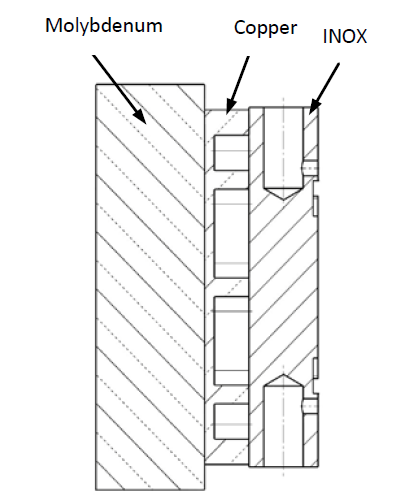
\includegraphics[width=0.45\textwidth]{LHC_Collimation_Upgrades/figures/mo-geo.png}
\label{fig:phase-2-moly}
}
\subfigure[]{
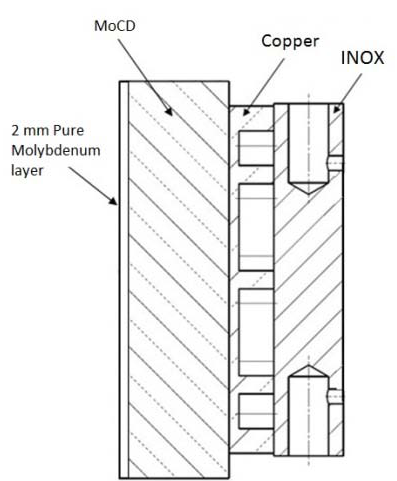
\includegraphics[width=0.45\textwidth]{LHC_Collimation_Upgrades/figures/mo-mocd-geo.png}
\label{fig:phase-2-molycd}
}
\label{fig:phase-2-jaw-designs}
\caption{A number of the proposed jaw designs for the phase 2 secondary collimators. \ref{fig:phase-2-moly} shows the jaw made entirely from molybdenum. Glidcop maybe substituted for molybdenum in this design. \ref{fig:phase-2-molycd} shows the jaw made from a mixture of molybdenum diamond composite with a 2mm coating of molybdenum on the surface. The composite ensure a mechanically strong jaw, whilst the coating screens the higher resistivity composite and provides a smooth surface on the beam-facing part of the jaw. In this case the composite maybe substituted with copper diamond composite, and likewise the coating may be replaced with GlidCop.}
\end{figure}


\begin{itemize}
\item{Introduction to the collimator upgrade project - Why are collimators important}
\begin{enumerate}
\item{The have two significant physical requirements - a rigid, sturdy material and must be placed very close to the beam}
\item{The first necessitated the use of graphite/carbon materials for the phase 1 collimators due to their survivability in the condition needed. The second means that the resistive wall impedance is very large}
\end{enumerate}
\item{Phase 2 collimator materials choice}
\begin{enumerate}
\item{Why a phase 2 collimator upgrade?}
\item{Summary of the material requirements and the available materials}
\item{Simple model used - simulations and comparison to analytical models}
\end{enumerate}
